% corresponds to IESA 2017-04-07 (Have Slides 12 & 13 been included?)


% 2019-03-25

\documentclass[10pt]{article}
\usepackage[T1]{fontenc}
\usepackage{amssymb}
\usepackage{amsmath}
\usepackage{graphicx}
% \begin{figure}[h]
% \centering
% \includegraphics[width=6.5in]{folder/photo.png}
% \caption{}
% \label{}
% \end{figure}



\usepackage{tikz}
\usetikzlibrary{arrows}
\usepackage{subfigure}
\usepackage{stackrel}
\usepackage{blindtext}

\usepackage{biblatex}
\addbibresource{library.bib}

\oddsidemargin=0.15in
\evensidemargin=0.15in
\topmargin=-.5in
\textheight=9in
\textwidth=6.25in

\usepackage[colorlinks=true,breaklinks,pdfpagemode=none,linkcolor=blue,citecolor=blue]{hyperref}

\usepackage{enumerate}
% \vspace{-6pt}
% \begin{itemize}
%     \setlength{\itemsep}{0pt}%
%     \setlength{\parskip}{0pt}%
%     \item Item 1
%     \item Item 2
%         \begin{itemize}
%             \setlength{\itemsep}{0pt}%
%             \setlength{\parskip}{0pt}%
%             \item Sublist Item 1
%             \item Sublist Item 2
%         \end{itemize}
%         \item Item 3
% \end{itemize}
% \vspace{-6pt}


\usepackage{enumitem}
\setlist{itemsep=0mm}

\usepackage{amsmath,amsfonts,amssymb,bm}


\begin{document}

   \noindent
   \begin{center}

   \hrulefill
   
   \vspace{5pt}
   
   \makebox[\textwidth]{ {\bf Energy Systems Analysis} \hfill  A.D. Smith 2019}
   \vspace{0pt}
   
   {\Large \hfill  Lecture 25.  
Sensitivity Analysis (SA) for Models
}
   \vspace{5pt}
   
  
   \hrulefill
   \end{center}
   
 {\color{darkgray}{\center{ \small{      ``SA is not concerned with what causes the output of the model to be what it is, but what the sources of variation in that output are.''
\\%[3pt]
\rightline{{\rm --- Andrea Saltelli \cite{Saltelli2008-zc}}}}}}}


\section{What is sensitivity analysis?}


Sensitivity analysis tells us how (or whether) a variation in one thing (a model input) causes variation in another thing (a model output). ``Sensitivity analysis is a technique for taking into account uncertainty that does not require estimates of probabilities.'' \cite{Goswami2007-hf}. In a broader sense:

\begin{description}
\item [\textbf{Sensitivity analysis}] is a quantitative method where the modeler ``studies the relationships between information flowing in and out of the model.'' \cite{Saltelli2009-tz}
\end{description}

\subsection{Derivatives and change}

Think all the way back to your first calculus course---what does a derivative actually mean? For a total derivative in two dimensions, it's describing how one variable changes \textit{given a very small change in the other variable}. 

Here, \textit{y} is a function of an independent variable \textit{x} and the slope is illustrated:

%\medskip
            \begin{figure}[h]
            \centering
            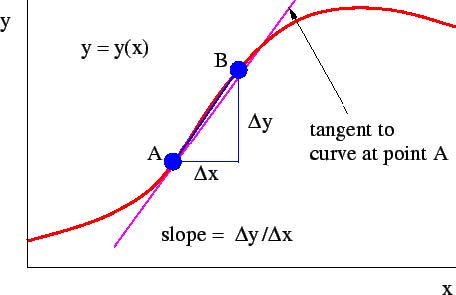
\includegraphics[width=6cm]{extras25/slope}
            \caption{Slope illustration from Wikipedia
            \label{slope}(\url{https://en.wikibooks.org/wiki/Waves/Derivatives})}
            \end{figure}
%\bigskip

The derivative is just a function that tells us how the slope changes as \textit{x} changes. When that `very small' {\color{blue}change becomes} so tiny it's infinitesimal, it looks like: $\frac{d y}{d x}$. When there are multiple parameters or ``factors'' in a model, sensitivities look like partial derivatives: $\frac{\partial y}{\partial x}$. These both describe the sensitivity of $y$ to a tiny change in $x$.

\subsection{Why perform SA?}
Why worry about finding a derivative and calling it sensitivity analysis? Saltelli 
\cite{Saltelli2009-tz} states that the goal of sensitivity analysis is to ``to apportion the variation in the output to the different sources of variation in the system.''\\

When performing a sensitivity analysis, we are asking questions like:

\vspace{-6pt}
\begin{itemize}
    \setlength{\itemsep}{0pt}%
    \setlength{\parskip}{0pt}%
    \item How much does this thing matter toward the outcomes I am interested in?
    \item When I change \textit{this} thing (e.g. \textit{x}), how much will change with \textit{that} thing (e.g. \textit{x})?
        \item How can I simplify my models without sacrificing their predictive power?
    \item How can I improve the predictive power of my models by strategically choosing where to focus my modeling efforts?
\end{itemize}
\vspace{-6pt}


Models improve because we keep asking questions.

\subsection{Compared with uncertainty analysis (UA)}

A sensitivity analysis itself does not have to address uncertainty, but in practice SA and UA are often performed together and may both be necessary for testing and understanding a particular model. Uncertainty is addressed in more detail in a {\color{blue}subsequent} lesson.

\section{An energy system example
}

\subsection{Y1: Simple linear response}

Let's say we have an empty room in a building that is initially held at $70\,^{\circ}\mathrm{F}$. Each additional occupant causes the temperature to rise by another $1\,^{\circ}\mathrm{F}$, as shown in Fig. \ref{Y1}.

%\medskip
            \begin{figure}[h]
            \centering
            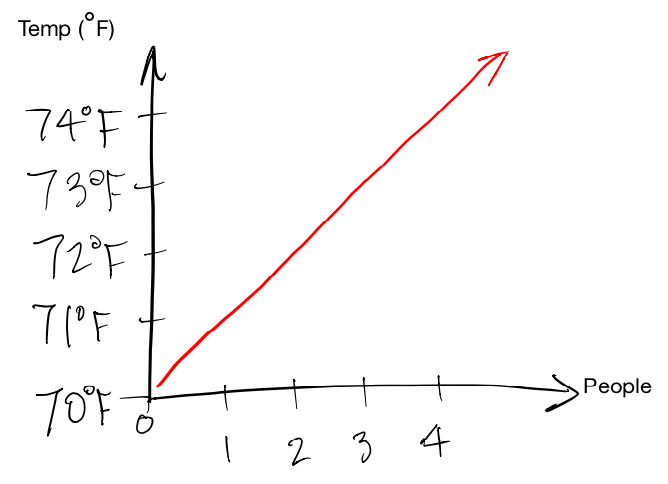
\includegraphics[width=4cm]{extras25/y1}
            \caption{Temperature response to occupancy increase, Y1}
            \label{Y1}
            \end{figure}
%\bigskip

Temperature here has a simple linear response. The derivative and the sensitivity of the temperature function with respect to the number of people present are the same:

$$\frac{\partial Y_1}{\partial x} =  \frac{1\,^{\circ}\mathrm{F}}{person}$$

The sensitivity remains the same throughout the process of adding people:

$$ S_{Y1} |_{x=1} &= S_{Y1}|_{x=3} $$

\subsection{Y2: Nonlinear response to interacting people}

We again have an empty room in a building that is initially $70\,^{\circ}\mathrm{F}$. However, we find that while the first occupant still causes the temperature to rise by $1\,^{\circ}\mathrm{F}$, additional occupants do not cause the same temperature response. As more people arrive, they interact with each other, becoming more animated and producing more body heat. So, Person 2, Person 3, and so on\ldots cause a greater rise in temperature then Person 1 did after joining the room, as shown in Fig. \ref{Y2}.

%\medskip
            \begin{figure}[h]
            \centering
            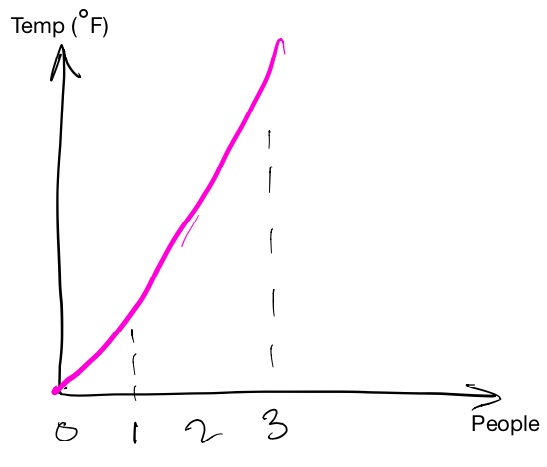
\includegraphics[width=3cm]{extras25/y2}
            \caption{Temperature response to occupancy increase, Y2}
            \label{Y2}
            \end{figure}
%\bigskip

Temperature here has a more dynamic response to additional occupants. The derivative and the sensitivity of the temperature function to the number of people will \textit{increase} as more people are added. The derivative is consistently positive, meaning that each person entering the room will cause an increase in temperature. It's just that Person 3 causes a \textit{bigger} increase in temperature than Person 1 did. That is to say, the sensitivity now changes throughout the process of adding people:

$$ S_{Y2} |_{x=1} \neq S_{Y2}|_{x=3} $$

\subsection{Y3: Nonlinear `diminishing returns'-type response}

We again have an empty room in a building that is initially $70\,^{\circ}\mathrm{F}$ and we still find that the first occupant  causes the temperature to rise by $1\,^{\circ}\mathrm{F}$. However, here we see that each subsequent occupant causes a slightly less dramatic temperature increase. The room's temperature will approach some maximum value, as shown in Fig. \ref{Y3}.

%\medskip
            \begin{figure}[h]
            \centering
            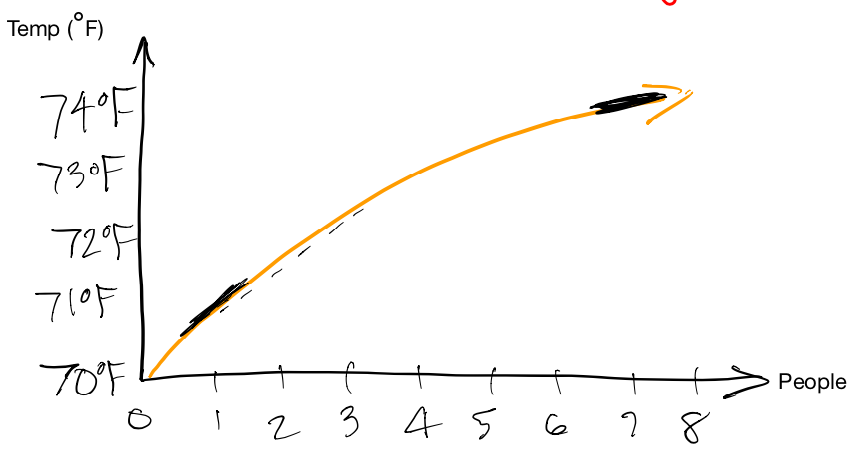
\includegraphics[width=4.5cm]{extras25/y3}
            \caption{Temperature response to occupancy increase, Y3}
            \label{Y3}
            \end{figure}
%\bigskip

Temperature here has a different response. The sensitivity of the temperature function with respect to the number of people will \textit{decrease} as more people are added--that is, the room's temperature is less sensitive to adding another person if there are already several people present. The derivative is still consistently positive (unless the temperature maxes out, in which case it would be zero), meaning that each person entering the room will cause an increase in temperature. It's just that Person 7 (see tangent line, right, in Fig. \ref{Y3}) causes a \textit{smaller} increase in temperature than Person 1 did (See tangent line, left, in Fig. \ref{Y3}). This means the impact of the first person is different than the impact of the third person or the seventh person, or any other person. That is to say, the sensitivity again changes throughout the process of adding people:

$$ S_{Y3} |_{x=1} \neq S_{Y3}|_{x=3} \neq S_{Y3}|_{x=7} $$

%\smallskip

Notice that in each case, Y1 to Y3, the sensitivity to Person 1 is the same. However, in function Y1 this sensitivity index is the same regardless of the number of occupants, while in functions Y2 and Y3 the sensitivity to an additional person will change based on the number of occupants.


% So what does a sensitivity number actually mean?

\section{How to perform a sensitivity analysis}

The following steps were adapted from Saltelli \cite{Saltelli2009-tz}:

\begin{enumerate}
    \setlength{\itemsep}{0pt}%
    \setlength{\parskip}{0pt}%
    \item Design the modeling experiment (identify what question the model should answer) and determine which of the input factors you are concerned with in the analysis.
    \item Assign a range of variation to each input factor (and a probability density function, if you have a known or estimated distribution).
    \item Evaluate the model, creating an output distribution for the response(s) of interest.
    \item Assess the influence or relative importance of each input factor you are concerned with on the output variable(s).
\end{enumerate}

In its simplest form, SA is the same as a \textit{parametric analysis}, where a certain parameter (factor) value is varied systematically to see how the output changes.

\section{Types of sensitivity}

We are always interested in how sensitive the model is \textit{to} something. That something may be:

\begin{itemize}
    \setlength{\itemsep}{0pt}%
    \setlength{\parskip}{0pt}%
    \item Parameter values
    \item Underlying distributions for input factors
    \item Assumptions or boundary conditions used in the model
    \item The structure of the model itself
\end{itemize}


\section{Simple sensitivity}

\subsection{General formulation}

The most straightforward way to define sensitivity is to use a \textit{local derivative}. Saltelli's expression \cite{Saltelli2008-zc} is shown below.

$$ S_x^d =  \frac{\partial Y}{\partial P_x} $$

where $s$ is the sensitivity of output $Y$ to factor $P$ at location `x' on $P$.\\
The `d' superscript denotes a dimensional sensitivity. It should be expressed with units attached to it (units for output Y divided by units for factor P).

\subsection{Normalized}

A normalized derivative may be useful in providing understanding about the relationships between input factors and output. An adapted version of Saltelli's expression \cite{Saltelli2008-zc} for this is shown below.

$$ S_x^\sigma =  \frac{\partial Y}{\partial P_x} \frac{\sigma_x}{\sigma_Y} $$

where $s$ is the sensitivity of output $Y$ to factor $P$ at location `x' on $P$, multiplied by the ratio of the standard deviation of the factor (at `x') to the standard deviation of the output.\\ 
The `$\sigma$' superscript denotes that the variance in both the output $Y$ and the factor $P$ at location `x' is taken into account. This results in a dimensionless quantity.

\subsection{Limitations} 

Since we have fixed the location where the sensitivity is quantified, the $S$ obtained in this way is only applicable when we are looking at `x' (unless we have a simple line, as in Fig. \ref{Y1}, but in that case we don't need to be doing a fancy SA!). The farther away we get from that location, and the more complex the model is (e.g. Y2 or Y3 v. Y1), the less useful that sensitivity index becomes. Because uncertainties in model inputs and nonlinear behaviors are confounding factors for a straightforward sensitivity analysis, we will see in future lectures why UA and \textit{global} SA are useful. 

% license
\medskip

\noindent
\texttt{\footnotesize RESTRICTED PUBLIC LICENSE --- READ BEFORE SHARING. This is a draft version made available by Amanda D. Smith under a Creative Commons Attribution-NonCommercial-ShareAlike license. 
\href{https://creativecommons.org/licenses/by-nc-sa/4.0/}{CC BY-NC-SA 4.0}}

% references
\printbibliography

\end{document}